\begin{frame}
  \frametitle{MD5}
  \begin{minipage}[t]{0.55\linewidth}
    % Points about MD5:
    \begin{itemize}
    \item Cryptograpic hash function
    \item Merkle-Damgaard construction
    \item Four different compression functions, 64 rounds
    \end{itemize}
  \end{minipage}\hfill
  \begin{minipage}[t][3cm][c]{0.45\linewidth}
    \centering
    \begin{figure}
      \centering
      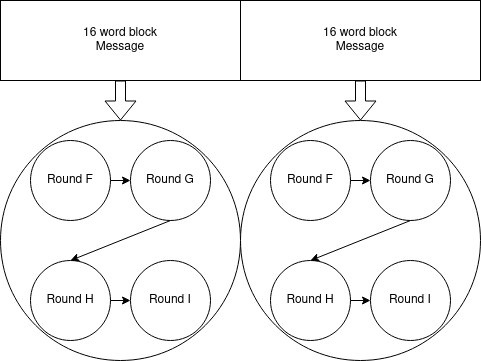
\includegraphics[width=\textwidth]{RoundsMD5}
      \caption{MD5 round}
    \end{figure}
  \end{minipage}

  \begin{minipage}[b][3.7cm][b]{0.9\linewidth}
    \begin{figure}
      \centering
      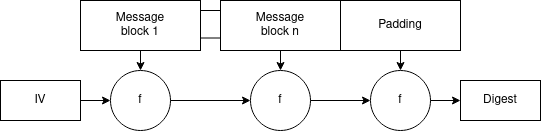
\includegraphics[width=0.95\textwidth]{merkle1}
      \caption{Merkle-Damgaard construction}
    \end{figure}
  \end{minipage}
\end{frame}

\begin{frame}
  \frametitle{MD5 - Optimizations}
  \begin{minipage}[t]{\linewidth}
    \begin{itemize}
    \item Naive; 1 simple process, 4 busses
    \item Pipelined version; clocked process for preprocessing and each compression stage
    \item Same idea for SHA-2
    \end{itemize}
  \end{minipage}\hfill
  \begin{minipage}[b]{\linewidth}
    \qquad
    \centering
    \begin{figure}
      \centering
      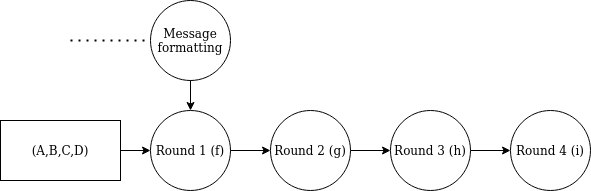
\includegraphics[width=0.85\textwidth]{md5}
      \caption{MD5 pipeline}
    \end{figure}
  \end{minipage}
\end{frame}

\begin{frame}
  \frametitle{MD5 - Pipeline}
  \begin{minipage}[t]{\textwidth}
    \begin{itemize}
    \item Stalls on large messages due to data dependency
    \item Solution is enabling multiple inputs
    \end{itemize}
  \end{minipage}
  \begin{minipage}[b]{\textwidth}
    \qquad
    \fontsize{8pt}{2}
    \selectfont
    \centering
    \begin{table}[H]
      \captionsetup{width=.8\linewidth}
      \centering
      \makebox[\linewidth]{
        \begin{tabular}{c c c c c c c c c c}
          \hline
          \multicolumn{10}{c}{Independent message blocks}\\
          \hline
          \textbf{clock} & 0   &  1  &  2  &  3  &  4   & 5 &  6 &  7 & 8\\
          \hline
                         & P$_1$ & M$_1$ & F$_1$ & G$_1$ & H$_1$  & I$_1$ & C$_1$ &  \\
                         &       & P$_2$ & M$_2$ & F$_2$ & G$_2$ & H$_2$  & I$_2$ & C$_2$ \\
        \end{tabular}
      }
      \newline
      \vspace*{0.5cm}
      \newline
      \centering
      \begin{tabular}{c c c c c c c c c c c c c}
        \hline
        \multicolumn{13}{c}{Dependent message blocks}\\
        \hline
        \textbf{clock} & 0   &  1  &  2  &  3  &  4   & 5 &  6 &     7 &    8  & 9   &    10  &    11\\
        \hline
                       & P$_1$ & M$_1$ & F$_1$ & G$_1$ & H$_1$  & I$_1$ & C$_1$ &     &        &         &       &     \\
                       &       & P$_2$ & M$_2$ &   -   &   -    &   -    &   -   & F$_2$ & G$_2$ & H$_2$  & I$_2$ & C$_2$ \\
      \end{tabular}
    \end{table}
  \end{minipage}
\end{frame}
